\documentclass[1p]{elsarticle_modified}
%\bibliographystyle{elsarticle-num}

%\usepackage[colorlinks]{hyperref}
%\usepackage{abbrmath_seonhwa} %\Abb, \Ascr, \Acal ,\Abf, \Afrak
\usepackage{amsfonts}
\usepackage{amssymb}
\usepackage{amsmath}
\usepackage{amsthm}
\usepackage{scalefnt}
\usepackage{amsbsy}
\usepackage{kotex}
\usepackage{caption}
\usepackage{subfig}
\usepackage{color}
\usepackage{graphicx}
\usepackage{xcolor} %% white, black, red, green, blue, cyan, magenta, yellow
\usepackage{float}
\usepackage{setspace}
\usepackage{hyperref}

\usepackage{tikz}
\usetikzlibrary{arrows}

\usepackage{multirow}
\usepackage{array} % fixed length table
\usepackage{hhline}

%%%%%%%%%%%%%%%%%%%%%
\makeatletter
\renewcommand*\env@matrix[1][\arraystretch]{%
	\edef\arraystretch{#1}%
	\hskip -\arraycolsep
	\let\@ifnextchar\new@ifnextchar
	\array{*\c@MaxMatrixCols c}}
\makeatother %https://tex.stackexchange.com/questions/14071/how-can-i-increase-the-line-spacing-in-a-matrix
%%%%%%%%%%%%%%%

\usepackage[normalem]{ulem}

\newcommand{\msout}[1]{\ifmmode\text{\sout{\ensuremath{#1}}}\else\sout{#1}\fi}
%SOURCE: \msout is \stkout macro in https://tex.stackexchange.com/questions/20609/strikeout-in-math-mode

\newcommand{\cancel}[1]{
	\ifmmode
	{\color{red}\msout{#1}}
	\else
	{\color{red}\sout{#1}}
	\fi
}

\newcommand{\add}[1]{
	{\color{blue}\uwave{#1}}
}

\newcommand{\replace}[2]{
	\ifmmode
	{\color{red}\msout{#1}}{\color{blue}\uwave{#2}}
	\else
	{\color{red}\sout{#1}}{\color{blue}\uwave{#2}}
	\fi
}

\newcommand{\Sol}{\mathcal{S}} %segment
\newcommand{\D}{D} %diagram
\newcommand{\A}{\mathcal{A}} %arc


%%%%%%%%%%%%%%%%%%%%%%%%%%%%%5 test

\def\sl{\operatorname{\textup{SL}}(2,\Cbb)}
\def\psl{\operatorname{\textup{PSL}}(2,\Cbb)}
\def\quan{\mkern 1mu \triangleright \mkern 1mu}

\theoremstyle{definition}
\newtheorem{thm}{Theorem}[section]
\newtheorem{prop}[thm]{Proposition}
\newtheorem{lem}[thm]{Lemma}
\newtheorem{ques}[thm]{Question}
\newtheorem{cor}[thm]{Corollary}
\newtheorem{defn}[thm]{Definition}
\newtheorem{exam}[thm]{Example}
\newtheorem{rmk}[thm]{Remark}
\newtheorem{alg}[thm]{Algorithm}

\newcommand{\I}{\sqrt{-1}}
\begin{document}

%\begin{frontmatter}
%
%\title{Boundary parabolic representations of knots up to 8 crossings}
%
%%% Group authors per affiliation:
%\author{Yunhi Cho} 
%\address{Department of Mathematics, University of Seoul, Seoul, Korea}
%\ead{yhcho@uos.ac.kr}
%
%
%\author{Seonhwa Kim} %\fnref{s_kim}}
%\address{Center for Geometry and Physics, Institute for Basic Science, Pohang, 37673, Korea}
%\ead{ryeona17@ibs.re.kr}
%
%\author{Hyuk Kim}
%\address{Department of Mathematical Sciences, Seoul National University, Seoul 08826, Korea}
%\ead{hyukkim@snu.ac.kr}
%
%\author{Seokbeom Yoon}
%\address{Department of Mathematical Sciences, Seoul National University, Seoul, 08826,  Korea}
%\ead{sbyoon15@snu.ac.kr}
%
%\begin{abstract}
%We find all boundary parabolic representation of knots up to 8 crossings.
%
%\end{abstract}
%\begin{keyword}
%    \MSC[2010] 57M25 
%\end{keyword}
%
%\end{frontmatter}

%\linenumbers
%\tableofcontents
%
\newcommand\colored[1]{\textcolor{white}{\rule[-0.35ex]{0.8em}{1.4ex}}\kern-0.8em\color{red} #1}%
%\newcommand\colored[1]{\textcolor{white}{ #1}\kern-2.17ex	\textcolor{white}{ #1}\kern-1.81ex	\textcolor{white}{ #1}\kern-2.15ex\color{red}#1	}

{\Large $\underline{12n_{0349}~(K12n_{0349})}$}

\setlength{\tabcolsep}{10pt}
\renewcommand{\arraystretch}{1.6}
\vspace{1cm}\begin{tabular}{m{100pt}>{\centering\arraybackslash}m{274pt}}
\multirow{5}{120pt}{
	\centering
	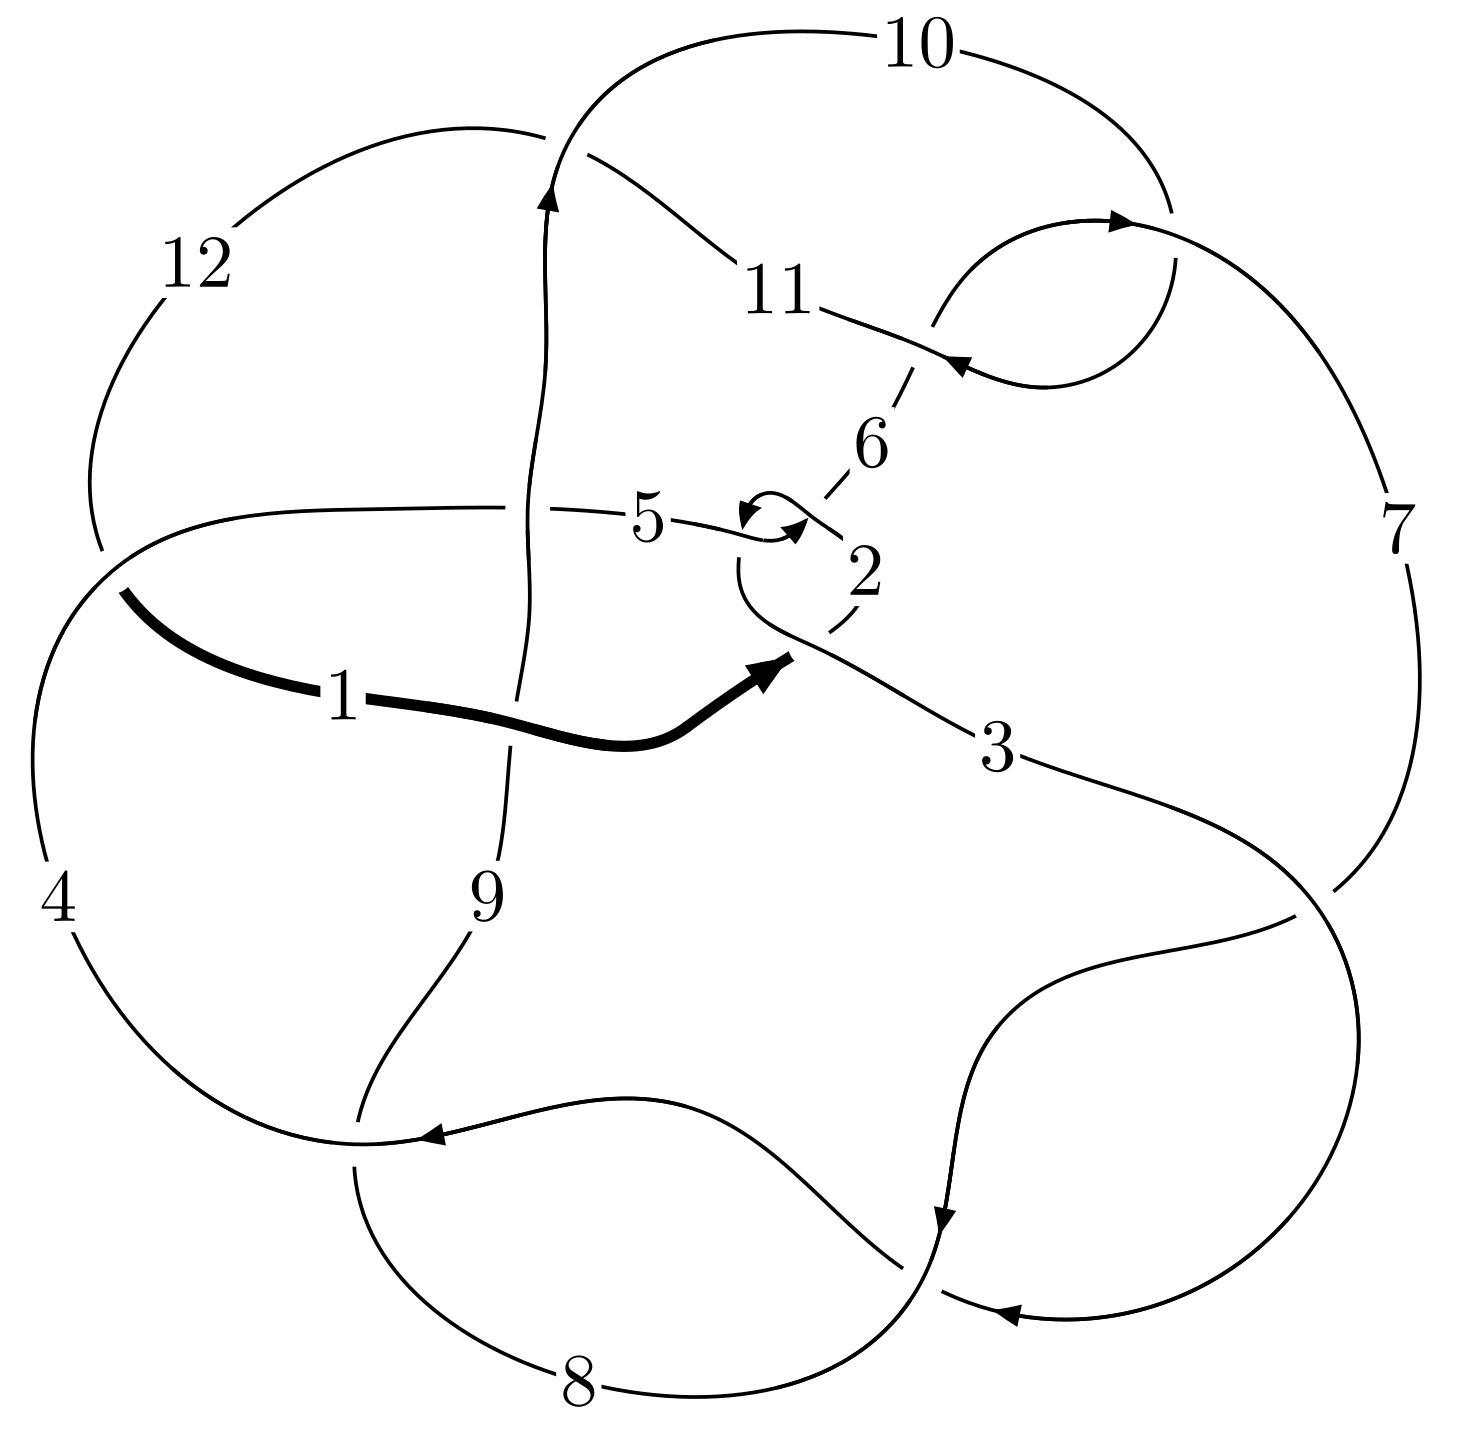
\includegraphics[width=112pt]{../../../GIT/diagram.site/Diagrams/png/2438_12n_0349.png}\\
\ \ \ A knot diagram\footnotemark}&
\allowdisplaybreaks
\textbf{Linearized knot diagam} \\
\cline{2-2}
 &
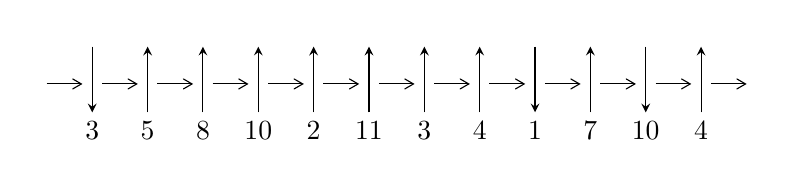
\begin{tikzpicture}[x=20pt, y=17pt]
	% nodes
	\node (C0) at (0, 0) {};
	\node (C1) at (1, 0) {};
	\node (C1U) at (1, +1) {};
	\node (C1D) at (1, -1) {3};

	\node (C2) at (2, 0) {};
	\node (C2U) at (2, +1) {};
	\node (C2D) at (2, -1) {5};

	\node (C3) at (3, 0) {};
	\node (C3U) at (3, +1) {};
	\node (C3D) at (3, -1) {8};

	\node (C4) at (4, 0) {};
	\node (C4U) at (4, +1) {};
	\node (C4D) at (4, -1) {10};

	\node (C5) at (5, 0) {};
	\node (C5U) at (5, +1) {};
	\node (C5D) at (5, -1) {2};

	\node (C6) at (6, 0) {};
	\node (C6U) at (6, +1) {};
	\node (C6D) at (6, -1) {11};

	\node (C7) at (7, 0) {};
	\node (C7U) at (7, +1) {};
	\node (C7D) at (7, -1) {3};

	\node (C8) at (8, 0) {};
	\node (C8U) at (8, +1) {};
	\node (C8D) at (8, -1) {4};

	\node (C9) at (9, 0) {};
	\node (C9U) at (9, +1) {};
	\node (C9D) at (9, -1) {1};

	\node (C10) at (10, 0) {};
	\node (C10U) at (10, +1) {};
	\node (C10D) at (10, -1) {7};

	\node (C11) at (11, 0) {};
	\node (C11U) at (11, +1) {};
	\node (C11D) at (11, -1) {10};

	\node (C12) at (12, 0) {};
	\node (C12U) at (12, +1) {};
	\node (C12D) at (12, -1) {4};
	\node (C13) at (13, 0) {};

	% arrows
	\draw[->,>={angle 60}]
	(C0) edge (C1) (C1) edge (C2) (C2) edge (C3) (C3) edge (C4) (C4) edge (C5) (C5) edge (C6) (C6) edge (C7) (C7) edge (C8) (C8) edge (C9) (C9) edge (C10) (C10) edge (C11) (C11) edge (C12) (C12) edge (C13) ;	\draw[->,>=stealth]
	(C1U) edge (C1D) (C2D) edge (C2U) (C3D) edge (C3U) (C4D) edge (C4U) (C5D) edge (C5U) (C6D) edge (C6U) (C7D) edge (C7U) (C8D) edge (C8U) (C9U) edge (C9D) (C10D) edge (C10U) (C11U) edge (C11D) (C12D) edge (C12U) ;
	\end{tikzpicture} \\
\hhline{~~} \\& 
\textbf{Solving Sequence} \\ \cline{2-2} 
 &
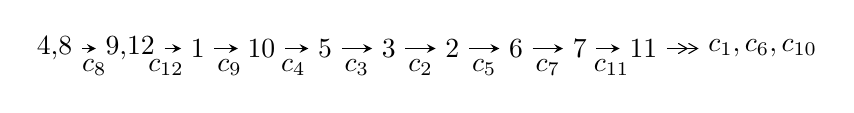
\begin{tikzpicture}[x=23pt, y=7pt]
	% node
	\node (A0) at (-1/8, 0) {4,8};
	\node (A1) at (17/16, 0) {9,12};
	\node (A2) at (17/8, 0) {1};
	\node (A3) at (25/8, 0) {10};
	\node (A4) at (33/8, 0) {5};
	\node (A5) at (41/8, 0) {3};
	\node (A6) at (49/8, 0) {2};
	\node (A7) at (57/8, 0) {6};
	\node (A8) at (65/8, 0) {7};
	\node (A9) at (73/8, 0) {11};
	\node (C1) at (1/2, -1) {$c_{8}$};
	\node (C2) at (13/8, -1) {$c_{12}$};
	\node (C3) at (21/8, -1) {$c_{9}$};
	\node (C4) at (29/8, -1) {$c_{4}$};
	\node (C5) at (37/8, -1) {$c_{3}$};
	\node (C6) at (45/8, -1) {$c_{2}$};
	\node (C7) at (53/8, -1) {$c_{5}$};
	\node (C8) at (61/8, -1) {$c_{7}$};
	\node (C9) at (69/8, -1) {$c_{11}$};
	\node (A10) at (11, 0) {$c_{1},c_{6},c_{10}$};

	% edge
	\draw[->,>=stealth]	
	(A0) edge (A1) (A1) edge (A2) (A2) edge (A3) (A3) edge (A4) (A4) edge (A5) (A5) edge (A6) (A6) edge (A7) (A7) edge (A8) (A8) edge (A9) ;
	\draw[->>,>={angle 60}]	
	(A9) edge (A10);
\end{tikzpicture} \\ 

\end{tabular} \\

\footnotetext{
The image of knot diagram is generated by the software ``\textbf{Draw programme}" developed by Andrew Bartholomew(\url{http://www.layer8.co.uk/maths/draw/index.htm\#Running-draw}), where we modified some parts for our purpose(\url{https://github.com/CATsTAILs/LinksPainter}).
}\phantom \\ \newline 
\centering \textbf{Ideals for irreducible components\footnotemark of $X_{\text{par}}$} 
 
\begin{align*}
I^u_{1}&=\langle 
5.03279\times10^{28} u^{21}+1.41088\times10^{28} u^{20}+\cdots+3.11126\times10^{30} b-1.47947\times10^{30},\\
\phantom{I^u_{1}}&\phantom{= \langle  }2.83952\times10^{29} u^{21}+2.39177\times10^{30} u^{20}+\cdots+5.38247\times10^{32} a-1.28920\times10^{33},\\
\phantom{I^u_{1}}&\phantom{= \langle  }u^{22}- u^{21}+\cdots+570 u-173\rangle \\
I^u_{2}&=\langle 
4 u^{15}+u^{14}+\cdots+b-5,\;5 u^{15}+2 u^{14}+\cdots+a-5,\\
\phantom{I^u_{2}}&\phantom{= \langle  }u^{16}-7 u^{14}- u^{13}+22 u^{12}+6 u^{11}-43 u^{10}-15 u^9+58 u^8+19 u^7-52 u^6-13 u^5+29 u^4+5 u^3-8 u^2- u+1\rangle \\
\\
\end{align*}
\raggedright * 2 irreducible components of $\dim_{\mathbb{C}}=0$, with total 38 representations.\\
\footnotetext{All coefficients of polynomials are rational numbers. But the coefficients are sometimes approximated in decimal forms when there is not enough margin.}
\newpage
\renewcommand{\arraystretch}{1}
\centering \section*{I. $I^u_{1}= \langle 5.03\times10^{28} u^{21}+1.41\times10^{28} u^{20}+\cdots+3.11\times10^{30} b-1.48\times10^{30},\;2.84\times10^{29} u^{21}+2.39\times10^{30} u^{20}+\cdots+5.38\times10^{32} a-1.29\times10^{33},\;u^{22}- u^{21}+\cdots+570 u-173 \rangle$}
\flushleft \textbf{(i) Arc colorings}\\
\begin{tabular}{m{7pt} m{180pt} m{7pt} m{180pt} }
\flushright $a_{4}=$&$\begin{pmatrix}0\\u\end{pmatrix}$ \\
\flushright $a_{8}=$&$\begin{pmatrix}1\\0\end{pmatrix}$ \\
\flushright $a_{9}=$&$\begin{pmatrix}1\\- u^2\end{pmatrix}$ \\
\flushright $a_{12}=$&$\begin{pmatrix}-0.000527549 u^{21}-0.00444362 u^{20}+\cdots-2.94596 u+2.39519\\-0.0161761 u^{21}-0.00453474 u^{20}+\cdots+4.84486 u+0.475523\end{pmatrix}$ \\
\flushright $a_{1}=$&$\begin{pmatrix}-0.000527549 u^{21}-0.00444362 u^{20}+\cdots-2.94596 u+2.39519\\-0.0112823 u^{21}-0.00307489 u^{20}+\cdots+2.10256 u+1.33554\end{pmatrix}$ \\
\flushright $a_{10}=$&$\begin{pmatrix}-0.00747297 u^{21}-0.00222999 u^{20}+\cdots+1.32872 u+0.919896\\-0.0287409 u^{21}+0.00951872 u^{20}+\cdots+15.0584 u-4.13187\end{pmatrix}$ \\
\flushright $a_{5}=$&$\begin{pmatrix}-0.0176760 u^{21}+0.00338113 u^{20}+\cdots+7.60759 u-1.52246\\-0.00312229 u^{21}+0.0168476 u^{20}+\cdots+9.58458 u-3.73734\end{pmatrix}$ \\
\flushright $a_{3}=$&$\begin{pmatrix}- u\\u\end{pmatrix}$ \\
\flushright $a_{2}=$&$\begin{pmatrix}0.0117801 u^{21}-0.0136133 u^{20}+\cdots-11.9200 u+5.73898\\-0.0235899 u^{21}+0.00609484 u^{20}+\cdots+11.0766 u-2.00826\end{pmatrix}$ \\
\flushright $a_{6}=$&$\begin{pmatrix}0.0114740 u^{21}-0.00633450 u^{20}+\cdots-6.51280 u+1.90552\\-0.0333527 u^{21}+0.0105246 u^{20}+\cdots+16.7996 u-4.51821\end{pmatrix}$ \\
\flushright $a_{7}=$&$\begin{pmatrix}- u^2+1\\u^2\end{pmatrix}$ \\
\flushright $a_{11}=$&$\begin{pmatrix}-0.0267510 u^{21}-0.00298230 u^{20}+\cdots+5.83060 u+2.41175\\-0.0193326 u^{21}+0.0165589 u^{20}+\cdots+15.3927 u-4.75155\end{pmatrix}$\\&\end{tabular}
\flushleft \textbf{(ii) Obstruction class $= -1$}\\~\\
\flushleft \textbf{(iii) Cusp Shapes $= 0.0344880 u^{21}-0.0647662 u^{20}+\cdots-54.7216 u+34.1950$}\\~\\
\newpage\renewcommand{\arraystretch}{1}
\flushleft \textbf{(iv) u-Polynomials at the component}\newline \\
\begin{tabular}{m{50pt}|m{274pt}}
Crossings & \hspace{64pt}u-Polynomials at each crossing \\
\hline $$\begin{aligned}c_{1}\end{aligned}$$&$\begin{aligned}
&u^{22}+3 u^{21}+\cdots+129 u+121
\end{aligned}$\\
\hline $$\begin{aligned}c_{2},c_{5}\end{aligned}$$&$\begin{aligned}
&u^{22}+3 u^{21}+\cdots+61 u-11
\end{aligned}$\\
\hline $$\begin{aligned}c_{3},c_{7},c_{8}\end{aligned}$$&$\begin{aligned}
&u^{22}+u^{21}+\cdots-570 u-173
\end{aligned}$\\
\hline $$\begin{aligned}c_{4}\end{aligned}$$&$\begin{aligned}
&u^{22}+12 u^{21}+\cdots-5056 u-1856
\end{aligned}$\\
\hline $$\begin{aligned}c_{6},c_{10}\end{aligned}$$&$\begin{aligned}
&u^{22}- u^{21}+\cdots+387 u-119
\end{aligned}$\\
\hline $$\begin{aligned}c_{9}\end{aligned}$$&$\begin{aligned}
&u^{22}-3 u^{21}+\cdots-17 u+1
\end{aligned}$\\
\hline $$\begin{aligned}c_{11}\end{aligned}$$&$\begin{aligned}
&u^{22}+u^{21}+\cdots-50523 u+14161
\end{aligned}$\\
\hline $$\begin{aligned}c_{12}\end{aligned}$$&$\begin{aligned}
&u^{22}+u^{21}+\cdots+8 u+1
\end{aligned}$\\
\hline
\end{tabular}\\~\\
\newpage\renewcommand{\arraystretch}{1}
\flushleft \textbf{(v) Riley Polynomials at the component}\newline \\
\begin{tabular}{m{50pt}|m{274pt}}
Crossings & \hspace{64pt}Riley Polynomials at each crossing \\
\hline $$\begin{aligned}c_{1}\end{aligned}$$&$\begin{aligned}
&y^{22}+47 y^{21}+\cdots+1408497 y+14641
\end{aligned}$\\
\hline $$\begin{aligned}c_{2},c_{5}\end{aligned}$$&$\begin{aligned}
&y^{22}+3 y^{21}+\cdots+129 y+121
\end{aligned}$\\
\hline $$\begin{aligned}c_{3},c_{7},c_{8}\end{aligned}$$&$\begin{aligned}
&y^{22}-33 y^{21}+\cdots-222830 y+29929
\end{aligned}$\\
\hline $$\begin{aligned}c_{4}\end{aligned}$$&$\begin{aligned}
&y^{22}-48 y^{21}+\cdots-17842176 y+3444736
\end{aligned}$\\
\hline $$\begin{aligned}c_{6},c_{10}\end{aligned}$$&$\begin{aligned}
&y^{22}+y^{21}+\cdots-50523 y+14161
\end{aligned}$\\
\hline $$\begin{aligned}c_{9}\end{aligned}$$&$\begin{aligned}
&y^{22}+17 y^{21}+\cdots-89 y+1
\end{aligned}$\\
\hline $$\begin{aligned}c_{11}\end{aligned}$$&$\begin{aligned}
&y^{22}+57 y^{21}+\cdots-20509146359 y+200533921
\end{aligned}$\\
\hline $$\begin{aligned}c_{12}\end{aligned}$$&$\begin{aligned}
&y^{22}+49 y^{21}+\cdots-52 y+1
\end{aligned}$\\
\hline
\end{tabular}\\~\\
\newpage\flushleft \textbf{(vi) Complex Volumes and Cusp Shapes}
$$\begin{array}{c|c|c}  
\text{Solutions to }I^u_{1}& \I (\text{vol} + \sqrt{-1}CS) & \text{Cusp shape}\\
 \hline 
\begin{aligned}
u &= \phantom{-}0.888889 + 0.621508 I \\
a &= -0.785790 - 0.787936 I \\
b &= \phantom{-}1.41234 - 0.32273 I\end{aligned}
 & -2.09331 + 2.22663 I & \phantom{-}10.35334 - 5.55870 I \\ \hline\begin{aligned}
u &= \phantom{-}0.888889 - 0.621508 I \\
a &= -0.785790 + 0.787936 I \\
b &= \phantom{-}1.41234 + 0.32273 I\end{aligned}
 & -2.09331 - 2.22663 I & \phantom{-}10.35334 + 5.55870 I \\ \hline\begin{aligned}
u &= \phantom{-}1.125980 + 0.181359 I \\
a &= \phantom{-}0.194049 + 0.934438 I \\
b &= \phantom{-}0.533838 + 1.294670 I\end{aligned}
 & \phantom{-}2.80761 - 4.32610 I & \phantom{-}7.93255 + 4.44451 I \\ \hline\begin{aligned}
u &= \phantom{-}1.125980 - 0.181359 I \\
a &= \phantom{-}0.194049 - 0.934438 I \\
b &= \phantom{-}0.533838 - 1.294670 I\end{aligned}
 & \phantom{-}2.80761 + 4.32610 I & \phantom{-}7.93255 - 4.44451 I \\ \hline\begin{aligned}
u &= \phantom{-}0.468073 + 0.568730 I \\
a &= \phantom{-}0.033725 - 0.194825 I \\
b &= \phantom{-}0.67213 + 1.29726 I\end{aligned}
 & \phantom{-}0.96204 - 3.13844 I & \phantom{-}5.33676 + 0.34451 I \\ \hline\begin{aligned}
u &= \phantom{-}0.468073 - 0.568730 I \\
a &= \phantom{-}0.033725 + 0.194825 I \\
b &= \phantom{-}0.67213 - 1.29726 I\end{aligned}
 & \phantom{-}0.96204 + 3.13844 I & \phantom{-}5.33676 - 0.34451 I \\ \hline\begin{aligned}
u &= -1.219380 + 0.529046 I \\
a &= -1.29654 + 1.66639 I \\
b &= \phantom{-}0.021894 + 0.717525 I\end{aligned}
 & -9.56729 - 1.76902 I & \phantom{-}9.41797 + 0.67359 I \\ \hline\begin{aligned}
u &= -1.219380 - 0.529046 I \\
a &= -1.29654 - 1.66639 I \\
b &= \phantom{-}0.021894 - 0.717525 I\end{aligned}
 & -9.56729 + 1.76902 I & \phantom{-}9.41797 - 0.67359 I \\ \hline\begin{aligned}
u &= \phantom{-}1.138980 + 0.705814 I \\
a &= \phantom{-}0.762830 + 0.903956 I \\
b &= -1.373520 + 0.140422 I\end{aligned}
 & -5.89358 + 2.47710 I & \phantom{-}2.52368 - 2.07081 I \\ \hline\begin{aligned}
u &= \phantom{-}1.138980 - 0.705814 I \\
a &= \phantom{-}0.762830 - 0.903956 I \\
b &= -1.373520 - 0.140422 I\end{aligned}
 & -5.89358 - 2.47710 I & \phantom{-}2.52368 + 2.07081 I\\
 \hline 
 \end{array}$$\newpage$$\begin{array}{c|c|c}  
\text{Solutions to }I^u_{1}& \I (\text{vol} + \sqrt{-1}CS) & \text{Cusp shape}\\
 \hline 
\begin{aligned}
u &= \phantom{-}0.390919 + 0.487203 I \\
a &= -0.142272 - 0.861639 I \\
b &= \phantom{-}0.433308 - 0.046954 I\end{aligned}
 & -1.67513 + 1.49906 I & \phantom{-}2.16861 - 5.00550 I \\ \hline\begin{aligned}
u &= \phantom{-}0.390919 - 0.487203 I \\
a &= -0.142272 + 0.861639 I \\
b &= \phantom{-}0.433308 + 0.046954 I\end{aligned}
 & -1.67513 - 1.49906 I & \phantom{-}2.16861 + 5.00550 I \\ \hline\begin{aligned}
u &= -0.486914\phantom{ +0.000000I} \\
a &= \phantom{-}0.684920\phantom{ +0.000000I} \\
b &= -0.232651\phantom{ +0.000000I}\end{aligned}
 & \phantom{-}0.667389\phantom{ +0.000000I} & \phantom{-}15.1430\phantom{ +0.000000I} \\ \hline\begin{aligned}
u &= -1.51784 + 0.10872 I \\
a &= \phantom{-}0.152442 + 0.390876 I \\
b &= -0.0746395 + 0.0560374 I\end{aligned}
 & \phantom{-}4.60852 - 3.54663 I & \phantom{-}3.76213 + 0.30741 I \\ \hline\begin{aligned}
u &= -1.51784 - 0.10872 I \\
a &= \phantom{-}0.152442 - 0.390876 I \\
b &= -0.0746395 - 0.0560374 I\end{aligned}
 & \phantom{-}4.60852 + 3.54663 I & \phantom{-}3.76213 - 0.30741 I \\ \hline\begin{aligned}
u &= -1.16828 + 1.29949 I \\
a &= \phantom{-}0.771799 - 0.429092 I \\
b &= -0.50715 - 2.09278 I\end{aligned}
 & \phantom{-}5.62161 - 3.04840 I & \phantom{-}8.24444 + 1.87699 I \\ \hline\begin{aligned}
u &= -1.16828 - 1.29949 I \\
a &= \phantom{-}0.771799 + 0.429092 I \\
b &= -0.50715 + 2.09278 I\end{aligned}
 & \phantom{-}5.62161 + 3.04840 I & \phantom{-}8.24444 - 1.87699 I \\ \hline\begin{aligned}
u &= \phantom{-}1.88865 + 0.65161 I \\
a &= \phantom{-}0.557638 + 0.987237 I \\
b &= -1.32425 + 1.66024 I\end{aligned}
 & \phantom{-}14.5063 + 11.3964 I & \phantom{-}7.17418 - 4.33997 I \\ \hline\begin{aligned}
u &= \phantom{-}1.88865 - 0.65161 I \\
a &= \phantom{-}0.557638 - 0.987237 I \\
b &= -1.32425 - 1.66024 I\end{aligned}
 & \phantom{-}14.5063 - 11.3964 I & \phantom{-}7.17418 + 4.33997 I \\ \hline\begin{aligned}
u &= \phantom{-}2.18883\phantom{ +0.000000I} \\
a &= -0.226088\phantom{ +0.000000I} \\
b &= -2.17979\phantom{ +0.000000I}\end{aligned}
 & \phantom{-}10.8028\phantom{ +0.000000I} & \phantom{-}8.45190\phantom{ +0.000000I}\\
 \hline 
 \end{array}$$\newpage$$\begin{array}{c|c|c}  
\text{Solutions to }I^u_{1}& \I (\text{vol} + \sqrt{-1}CS) & \text{Cusp shape}\\
 \hline 
\begin{aligned}
u &= -2.34694 + 0.29798 I \\
a &= \phantom{-}0.184555 - 0.987184 I \\
b &= -0.08772 - 2.56787 I\end{aligned}
 & \phantom{-}16.2419 - 0.6601 I & \phantom{-}8.28889 + 0. I\phantom{ +0.000000I} \\ \hline\begin{aligned}
u &= -2.34694 - 0.29798 I \\
a &= \phantom{-}0.184555 + 0.987184 I \\
b &= -0.08772 + 2.56787 I\end{aligned}
 & \phantom{-}16.2419 + 0.6601 I & \phantom{-}8.28889 + 0. I\phantom{ +0.000000I}\\
 \hline 
 \end{array}$$\newpage\newpage\renewcommand{\arraystretch}{1}
\centering \section*{II. $I^u_{2}= \langle 4 u^{15}+u^{14}+\cdots+b-5,\;5 u^{15}+2 u^{14}+\cdots+a-5,\;u^{16}-7 u^{14}+\cdots- u+1 \rangle$}
\flushleft \textbf{(i) Arc colorings}\\
\begin{tabular}{m{7pt} m{180pt} m{7pt} m{180pt} }
\flushright $a_{4}=$&$\begin{pmatrix}0\\u\end{pmatrix}$ \\
\flushright $a_{8}=$&$\begin{pmatrix}1\\0\end{pmatrix}$ \\
\flushright $a_{9}=$&$\begin{pmatrix}1\\- u^2\end{pmatrix}$ \\
\flushright $a_{12}=$&$\begin{pmatrix}-5 u^{15}-2 u^{14}+\cdots+10 u+5\\-4 u^{15}- u^{14}+\cdots+9 u+5\end{pmatrix}$ \\
\flushright $a_{1}=$&$\begin{pmatrix}-5 u^{15}-2 u^{14}+\cdots+10 u+5\\-2 u^{15}+14 u^{13}+\cdots+6 u+3\end{pmatrix}$ \\
\flushright $a_{10}=$&$\begin{pmatrix}- u^{14}+6 u^{12}+\cdots-8 u^2- u\\-4 u^{15}-2 u^{14}+\cdots+7 u+6\end{pmatrix}$ \\
\flushright $a_{5}=$&$\begin{pmatrix}2 u^{15}-13 u^{13}+\cdots+3 u^2-2 u\\2 u^{15}+u^{14}+\cdots-2 u-5\end{pmatrix}$ \\
\flushright $a_{3}=$&$\begin{pmatrix}- u\\u\end{pmatrix}$ \\
\flushright $a_{2}=$&$\begin{pmatrix}-3 u^{15}- u^{14}+\cdots+5 u+3\\-4 u^{15}- u^{14}+\cdots+11 u+5\end{pmatrix}$ \\
\flushright $a_{6}=$&$\begin{pmatrix}5 u^{15}+u^{14}+\cdots-12 u-5\\4 u^{15}+2 u^{14}+\cdots-10 u-6\end{pmatrix}$ \\
\flushright $a_{7}=$&$\begin{pmatrix}- u^2+1\\u^2\end{pmatrix}$ \\
\flushright $a_{11}=$&$\begin{pmatrix}-2 u^{15}-2 u^{14}+\cdots+3 u+2\\-5 u^{15}-2 u^{14}+\cdots+9 u+7\end{pmatrix}$\\&\end{tabular}
\flushleft \textbf{(ii) Obstruction class $= 1$}\\~\\
\flushleft \textbf{(iii) Cusp Shapes $= -14 u^{15}-7 u^{14}+93 u^{13}+59 u^{12}-272 u^{11}-213 u^{10}+485 u^9+439 u^8-583 u^7-544 u^6+451 u^5+409 u^4-202 u^3-183 u^2+22 u+36$}\\~\\
\newpage\renewcommand{\arraystretch}{1}
\flushleft \textbf{(iv) u-Polynomials at the component}\newline \\
\begin{tabular}{m{50pt}|m{274pt}}
Crossings & \hspace{64pt}u-Polynomials at each crossing \\
\hline $$\begin{aligned}c_{1}\end{aligned}$$&$\begin{aligned}
&u^{16}-14 u^{15}+\cdots-18 u+1
\end{aligned}$\\
\hline $$\begin{aligned}c_{2}\end{aligned}$$&$\begin{aligned}
&u^{16}+2 u^{15}+\cdots+2 u+1
\end{aligned}$\\
\hline $$\begin{aligned}c_{3}\end{aligned}$$&$\begin{aligned}
&u^{16}-7 u^{14}+\cdots+u+1
\end{aligned}$\\
\hline $$\begin{aligned}c_{4}\end{aligned}$$&$\begin{aligned}
&u^{16}+2 u^{14}+\cdots- u+1
\end{aligned}$\\
\hline $$\begin{aligned}c_{5}\end{aligned}$$&$\begin{aligned}
&u^{16}-2 u^{15}+\cdots-2 u+1
\end{aligned}$\\
\hline $$\begin{aligned}c_{6}\end{aligned}$$&$\begin{aligned}
&u^{16}+8 u^{14}+\cdots+2 u+1
\end{aligned}$\\
\hline $$\begin{aligned}c_{7},c_{8}\end{aligned}$$&$\begin{aligned}
&u^{16}-7 u^{14}+\cdots- u+1
\end{aligned}$\\
\hline $$\begin{aligned}c_{9}\end{aligned}$$&$\begin{aligned}
&u^{16}-4 u^{15}+\cdots+4 u^3+1
\end{aligned}$\\
\hline $$\begin{aligned}c_{10}\end{aligned}$$&$\begin{aligned}
&u^{16}+8 u^{14}+\cdots-2 u+1
\end{aligned}$\\
\hline $$\begin{aligned}c_{11}\end{aligned}$$&$\begin{aligned}
&u^{16}+16 u^{15}+\cdots+18 u+1
\end{aligned}$\\
\hline $$\begin{aligned}c_{12}\end{aligned}$$&$\begin{aligned}
&u^{16}+14 u^{14}+\cdots+7 u+7
\end{aligned}$\\
\hline
\end{tabular}\\~\\
\newpage\renewcommand{\arraystretch}{1}
\flushleft \textbf{(v) Riley Polynomials at the component}\newline \\
\begin{tabular}{m{50pt}|m{274pt}}
Crossings & \hspace{64pt}Riley Polynomials at each crossing \\
\hline $$\begin{aligned}c_{1}\end{aligned}$$&$\begin{aligned}
&y^{16}-10 y^{15}+\cdots-42 y+1
\end{aligned}$\\
\hline $$\begin{aligned}c_{2},c_{5}\end{aligned}$$&$\begin{aligned}
&y^{16}+14 y^{15}+\cdots+18 y+1
\end{aligned}$\\
\hline $$\begin{aligned}c_{3},c_{7},c_{8}\end{aligned}$$&$\begin{aligned}
&y^{16}-14 y^{15}+\cdots-17 y+1
\end{aligned}$\\
\hline $$\begin{aligned}c_{4}\end{aligned}$$&$\begin{aligned}
&y^{16}+4 y^{15}+\cdots+y+1
\end{aligned}$\\
\hline $$\begin{aligned}c_{6},c_{10}\end{aligned}$$&$\begin{aligned}
&y^{16}+16 y^{15}+\cdots+18 y+1
\end{aligned}$\\
\hline $$\begin{aligned}c_{9}\end{aligned}$$&$\begin{aligned}
&y^{16}-4 y^{15}+\cdots-12 y^2+1
\end{aligned}$\\
\hline $$\begin{aligned}c_{11}\end{aligned}$$&$\begin{aligned}
&y^{16}-16 y^{15}+\cdots-18 y+1
\end{aligned}$\\
\hline $$\begin{aligned}c_{12}\end{aligned}$$&$\begin{aligned}
&y^{16}+28 y^{15}+\cdots+1505 y+49
\end{aligned}$\\
\hline
\end{tabular}\\~\\
\newpage\flushleft \textbf{(vi) Complex Volumes and Cusp Shapes}
$$\begin{array}{c|c|c}  
\text{Solutions to }I^u_{2}& \I (\text{vol} + \sqrt{-1}CS) & \text{Cusp shape}\\
 \hline 
\begin{aligned}
u &= \phantom{-}0.895121 + 0.512839 I \\
a &= -0.764453 - 0.786216 I \\
b &= \phantom{-}1.48200 - 0.38704 I\end{aligned}
 & -2.57741 + 2.02646 I & -4.32270 - 0.49641 I \\ \hline\begin{aligned}
u &= \phantom{-}0.895121 - 0.512839 I \\
a &= -0.764453 + 0.786216 I \\
b &= \phantom{-}1.48200 + 0.38704 I\end{aligned}
 & -2.57741 - 2.02646 I & -4.32270 + 0.49641 I \\ \hline\begin{aligned}
u &= -0.991446 + 0.300154 I \\
a &= \phantom{-}0.72110 - 1.52416 I \\
b &= -1.200410 - 0.280363 I\end{aligned}
 & -5.52393 - 1.17654 I & \phantom{-}4.37675 - 1.28594 I \\ \hline\begin{aligned}
u &= -0.991446 - 0.300154 I \\
a &= \phantom{-}0.72110 + 1.52416 I \\
b &= -1.200410 + 0.280363 I\end{aligned}
 & -5.52393 + 1.17654 I & \phantom{-}4.37675 + 1.28594 I \\ \hline\begin{aligned}
u &= \phantom{-}1.042540 + 0.498206 I \\
a &= \phantom{-}1.57083 + 2.03165 I \\
b &= -0.562512 + 0.129135 I\end{aligned}
 & -10.21970 + 1.92477 I & -2.98411 - 3.89934 I \\ \hline\begin{aligned}
u &= \phantom{-}1.042540 - 0.498206 I \\
a &= \phantom{-}1.57083 - 2.03165 I \\
b &= -0.562512 - 0.129135 I\end{aligned}
 & -10.21970 - 1.92477 I & -2.98411 + 3.89934 I \\ \hline\begin{aligned}
u &= -0.947353 + 0.893061 I \\
a &= -0.995021 + 0.545877 I \\
b &= \phantom{-}1.157010 + 0.171797 I\end{aligned}
 & -5.04353 - 3.27906 I & \phantom{-}6.96610 + 5.21245 I \\ \hline\begin{aligned}
u &= -0.947353 - 0.893061 I \\
a &= -0.995021 - 0.545877 I \\
b &= \phantom{-}1.157010 - 0.171797 I\end{aligned}
 & -5.04353 + 3.27906 I & \phantom{-}6.96610 - 5.21245 I \\ \hline\begin{aligned}
u &= -0.535533 + 0.224627 I \\
a &= -0.50673 - 1.96194 I \\
b &= \phantom{-}0.091098 - 1.093350 I\end{aligned}
 & \phantom{-}0.313495 - 1.189950 I & \phantom{-}7.79460 + 1.38246 I \\ \hline\begin{aligned}
u &= -0.535533 - 0.224627 I \\
a &= -0.50673 + 1.96194 I \\
b &= \phantom{-}0.091098 + 1.093350 I\end{aligned}
 & \phantom{-}0.313495 + 1.189950 I & \phantom{-}7.79460 - 1.38246 I\\
 \hline 
 \end{array}$$\newpage$$\begin{array}{c|c|c}  
\text{Solutions to }I^u_{2}& \I (\text{vol} + \sqrt{-1}CS) & \text{Cusp shape}\\
 \hline 
\begin{aligned}
u &= -1.42936 + 0.19543 I \\
a &= \phantom{-}0.667578 + 0.371646 I \\
b &= -0.005180 + 0.635975 I\end{aligned}
 & \phantom{-}3.92703 - 0.68720 I & \phantom{-}9.16301 - 0.40551 I \\ \hline\begin{aligned}
u &= -1.42936 - 0.19543 I \\
a &= \phantom{-}0.667578 - 0.371646 I \\
b &= -0.005180 - 0.635975 I\end{aligned}
 & \phantom{-}3.92703 + 0.68720 I & \phantom{-}9.16301 + 0.40551 I \\ \hline\begin{aligned}
u &= \phantom{-}1.46404 + 0.03561 I \\
a &= \phantom{-}0.004983 - 0.187762 I \\
b &= \phantom{-}0.403326 - 0.712059 I\end{aligned}
 & \phantom{-}5.03010 + 4.12297 I & \phantom{-}11.6031 - 8.8115 I \\ \hline\begin{aligned}
u &= \phantom{-}1.46404 - 0.03561 I \\
a &= \phantom{-}0.004983 + 0.187762 I \\
b &= \phantom{-}0.403326 + 0.712059 I\end{aligned}
 & \phantom{-}5.03010 - 4.12297 I & \phantom{-}11.6031 + 8.8115 I \\ \hline\begin{aligned}
u &= \phantom{-}0.501986 + 0.071058 I \\
a &= -0.69829 - 1.53708 I \\
b &= \phantom{-}0.634668 - 1.218490 I\end{aligned}
 & \phantom{-}0.93447 + 4.27246 I & \phantom{-}4.40321 - 6.78367 I \\ \hline\begin{aligned}
u &= \phantom{-}0.501986 - 0.071058 I \\
a &= -0.69829 + 1.53708 I \\
b &= \phantom{-}0.634668 + 1.218490 I\end{aligned}
 & \phantom{-}0.93447 - 4.27246 I & \phantom{-}4.40321 + 6.78367 I\\
 \hline 
 \end{array}$$\newpage
\newpage\renewcommand{\arraystretch}{1}
\centering \section*{ III. u-Polynomials}
\begin{tabular}{m{50pt}|m{274pt}}
Crossings & \hspace{64pt}u-Polynomials at each crossing \\
\hline $$\begin{aligned}c_{1}\end{aligned}$$&$\begin{aligned}
&(u^{16}-14 u^{15}+\cdots-18 u+1)(u^{22}+3 u^{21}+\cdots+129 u+121)
\end{aligned}$\\
\hline $$\begin{aligned}c_{2}\end{aligned}$$&$\begin{aligned}
&(u^{16}+2 u^{15}+\cdots+2 u+1)(u^{22}+3 u^{21}+\cdots+61 u-11)
\end{aligned}$\\
\hline $$\begin{aligned}c_{3}\end{aligned}$$&$\begin{aligned}
&(u^{16}-7 u^{14}+\cdots+u+1)(u^{22}+u^{21}+\cdots-570 u-173)
\end{aligned}$\\
\hline $$\begin{aligned}c_{4}\end{aligned}$$&$\begin{aligned}
&(u^{16}+2 u^{14}+\cdots- u+1)(u^{22}+12 u^{21}+\cdots-5056 u-1856)
\end{aligned}$\\
\hline $$\begin{aligned}c_{5}\end{aligned}$$&$\begin{aligned}
&(u^{16}-2 u^{15}+\cdots-2 u+1)(u^{22}+3 u^{21}+\cdots+61 u-11)
\end{aligned}$\\
\hline $$\begin{aligned}c_{6}\end{aligned}$$&$\begin{aligned}
&(u^{16}+8 u^{14}+\cdots+2 u+1)(u^{22}- u^{21}+\cdots+387 u-119)
\end{aligned}$\\
\hline $$\begin{aligned}c_{7},c_{8}\end{aligned}$$&$\begin{aligned}
&(u^{16}-7 u^{14}+\cdots- u+1)(u^{22}+u^{21}+\cdots-570 u-173)
\end{aligned}$\\
\hline $$\begin{aligned}c_{9}\end{aligned}$$&$\begin{aligned}
&(u^{16}-4 u^{15}+\cdots+4 u^3+1)(u^{22}-3 u^{21}+\cdots-17 u+1)
\end{aligned}$\\
\hline $$\begin{aligned}c_{10}\end{aligned}$$&$\begin{aligned}
&(u^{16}+8 u^{14}+\cdots-2 u+1)(u^{22}- u^{21}+\cdots+387 u-119)
\end{aligned}$\\
\hline $$\begin{aligned}c_{11}\end{aligned}$$&$\begin{aligned}
&(u^{16}+16 u^{15}+\cdots+18 u+1)(u^{22}+u^{21}+\cdots-50523 u+14161)
\end{aligned}$\\
\hline $$\begin{aligned}c_{12}\end{aligned}$$&$\begin{aligned}
&(u^{16}+14 u^{14}+\cdots+7 u+7)(u^{22}+u^{21}+\cdots+8 u+1)
\end{aligned}$\\
\hline
\end{tabular}\newpage\renewcommand{\arraystretch}{1}
\centering \section*{ IV. Riley Polynomials}
\begin{tabular}{m{50pt}|m{274pt}}
Crossings & \hspace{64pt}Riley Polynomials at each crossing \\
\hline $$\begin{aligned}c_{1}\end{aligned}$$&$\begin{aligned}
&(y^{16}-10 y^{15}+\cdots-42 y+1)(y^{22}+47 y^{21}+\cdots+1408497 y+14641)
\end{aligned}$\\
\hline $$\begin{aligned}c_{2},c_{5}\end{aligned}$$&$\begin{aligned}
&(y^{16}+14 y^{15}+\cdots+18 y+1)(y^{22}+3 y^{21}+\cdots+129 y+121)
\end{aligned}$\\
\hline $$\begin{aligned}c_{3},c_{7},c_{8}\end{aligned}$$&$\begin{aligned}
&(y^{16}-14 y^{15}+\cdots-17 y+1)(y^{22}-33 y^{21}+\cdots-222830 y+29929)
\end{aligned}$\\
\hline $$\begin{aligned}c_{4}\end{aligned}$$&$\begin{aligned}
&(y^{16}+4 y^{15}+\cdots+y+1)(y^{22}-48 y^{21}+\cdots-1.78422\times10^{7} y+3444736)
\end{aligned}$\\
\hline $$\begin{aligned}c_{6},c_{10}\end{aligned}$$&$\begin{aligned}
&(y^{16}+16 y^{15}+\cdots+18 y+1)(y^{22}+y^{21}+\cdots-50523 y+14161)
\end{aligned}$\\
\hline $$\begin{aligned}c_{9}\end{aligned}$$&$\begin{aligned}
&(y^{16}-4 y^{15}+\cdots-12 y^2+1)(y^{22}+17 y^{21}+\cdots-89 y+1)
\end{aligned}$\\
\hline $$\begin{aligned}c_{11}\end{aligned}$$&$\begin{aligned}
&(y^{16}-16 y^{15}+\cdots-18 y+1)\\
&\cdot(y^{22}+57 y^{21}+\cdots-20509146359 y+200533921)
\end{aligned}$\\
\hline $$\begin{aligned}c_{12}\end{aligned}$$&$\begin{aligned}
&(y^{16}+28 y^{15}+\cdots+1505 y+49)(y^{22}+49 y^{21}+\cdots-52 y+1)
\end{aligned}$\\
\hline
\end{tabular}
\vskip 2pc
\end{document}